%===================================================================================
% JORNADA CIENTÍFICA ESTUDIANTIL - MATCOM, UH
%===================================================================================
% Esta plantilla ha sido diseñada para ser usada en los artículos de la
% Jornada Científica Estudiantil, MatCom.
%
% Por favor, siga las instrucciones de esta plantilla y rellene en las secciones
% correspondientes.
%
% NOTA: Necesitará el archivo 'jcematcom.sty' en la misma carpeta donde esté este
%       archivo para poder utilizar esta plantila.
%===================================================================================



%===================================================================================
% PREÁMBULO
%-----------------------------------------------------------------------------------
\documentclass[a4paper,10pt,twocolumn]{article}

%===================================================================================
% Paquetes
%-----------------------------------------------------------------------------------
\usepackage{amsmath}
\usepackage{amsfonts}
\usepackage{amssymb}
\usepackage{jcematcom}
\usepackage[utf8]{inputenc}
\usepackage{listings}
\usepackage[pdftex]{hyperref}
\usepackage[x11names,table]{xcolor}
\usepackage{graphicx}
\usepackage{float}
%-----------------------------------------------------------------------------------
% Configuración
%-----------------------------------------------------------------------------------
\hypersetup{colorlinks,%
	    citecolor=black,%
	    filecolor=black,%
	    linkcolor=black,%
	    urlcolor=blue}

%===================================================================================



%===================================================================================
% Presentacion
%-----------------------------------------------------------------------------------
% Título
%-----------------------------------------------------------------------------------
\title{Proyecto de Estadística Fase 2}

%-----------------------------------------------------------------------------------
% Autores
%-----------------------------------------------------------------------------------
\author{\\
\name Enrique Martínez González \email \href{mailto:enrique.martinez@estudiantes.matcom.uh.cu}{enrique.martinez@estudiantes.matcom.uh.cu}
	\\ \addr Grupo C412 \AND
\name Osmany Pérez Rodríguez \email \href{mailto:osmany.perez@estudiantes.matcom.uh.cu}{osmany.perez@estudiantes.matcom.uh.cu}
  \\ \addr Grupo C412 \AND
\name Carmen Irene Cabrera Rodríguez \email \href{mailto:carmen.cabrera@estudiantes.matcom.uh.cu}{carmen.cabrera@estudiantes.matcom.uh.cu}
\\ \addr Grupo C412}

%-----------------------------------------------------------------------------------
% Tutores
%-----------------------------------------------------------------------------------
%\tutors{\\
%Dr. Tutor Uno, \emph{Centro} \\
%Lic. Tutor Dos, \emph{Centro}}

%-----------------------------------------------------------------------------------
% Headings
%-----------------------------------------------------------------------------------
\jcematcomheading{\the\year}{1-\pageref{end}}{E. Martínez, O. Pérez, C.Cabrera}

%-----------------------------------------------------------------------------------
\ShortHeadings{Proyecto de Estadística Fase 2}{Autores}
%===================================================================================



%===================================================================================
% DOCUMENTO
%-----------------------------------------------------------------------------------
\begin{document}

%-----------------------------------------------------------------------------------
% NO BORRAR ESTA LINEA!
%-----------------------------------------------------------------------------------
\twocolumn[
%-----------------------------------------------------------------------------------

\maketitle

%===================================================================================
% Resumen y Abstract
%-----------------------------------------------------------------------------------
\selectlanguage{spanish} % Para producir el documento en Español

%-----------------------------------------------------------------------------------
% Resumen en Español
%-----------------------------------------------------------------------------------


%-----------------------------------------------------------------------------------
% English Abstract
%-----------------------------------------------------------------------------------

%-----------------------------------------------------------------------------------
% Temas
%-----------------------------------------------------------------------------------



%-----------------------------------------------------------------------------------
% NO BORRAR ESTAS LINEAS!
%-----------------------------------------------------------------------------------
\vspace{0.8cm}
]
%-----------------------------------------------------------------------------------


%===================================================================================

%===================================================================================
% Introducción
%-----------------------------------------------------------------------------------
\section{Introducción}\label{sec:intro}
%-----------------------------------------------------------------------------------
%===================================================================================



%===================================================================================
% Desarrollo
%-----------------------------------------------------------------------------------
\section{Reducción de dimensión}\label{sec:ex1}
%-----------------------------------------------------------------------------------
	Nuestro set de datos posee un total de 145 variables, el cual es un número bastante grande  para intentar graficar todas las variables para apreciar a simple vista si los datos están correlacionados o no, de igual forma la matriz de correlación sigue siendo bastante grande pero podemos ver que muy pocos datos tienen correlación entre si. Intentando disminuir la cantidad de variables realizamos ACP pero dado los resultados anteriores esta no es altamente correlacionada por lo que habría que tomar un número igual grande de componentes principales para poder representar un \% no tan grande de la muestra.

	Intentemos agrupar los datos mediante el algoritmo de clusters jerárquico. Para esto el primer paso es estandarizar las muestras para evitar errores de clasificación. Los resultados arrojados los podemos apreciar en la gráfica \ref{fig:dendograma_1}, en estos se ve como todos los datos son semejantes, esto se debe al alto número de variables y la poca correlación que existe entre ellas imposibilitando agrupar los datos en clusters.

	\begin{figure}[htb]
		\begin{center}
			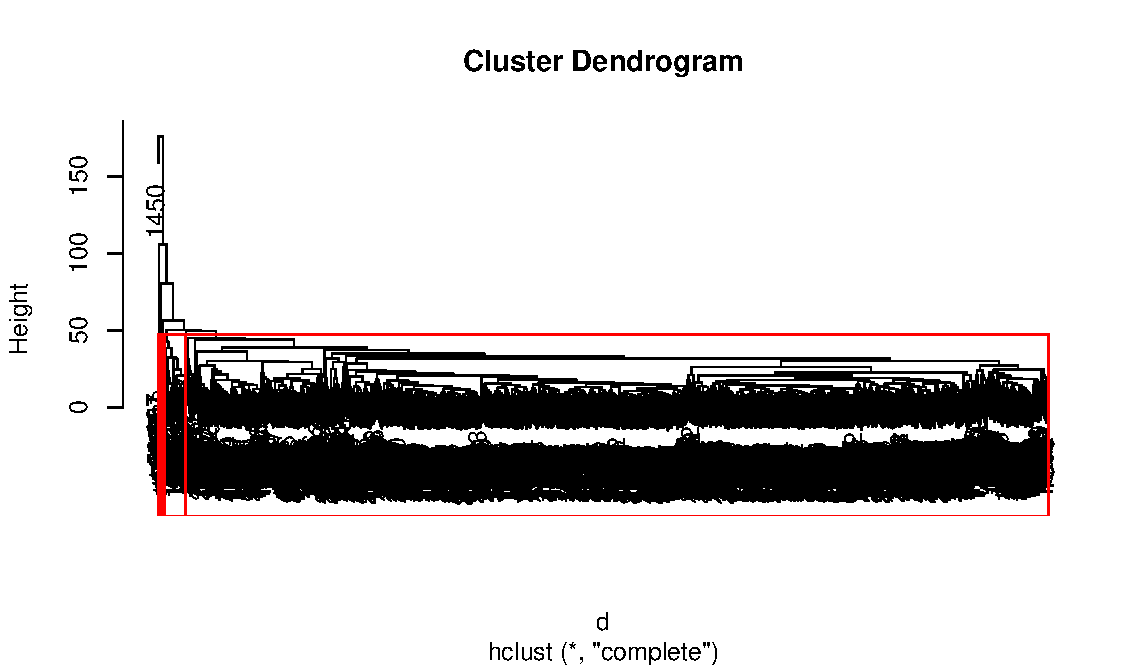
\includegraphics[width=\columnwidth]{figures/dendograma_1.pdf}
		\end{center}
		\caption{clusters jerárquico de los datos con todas las variables \label{fig:dendograma_1}}%
	\end{figure}

	Para aplicar el algoritmo de K-Means debemos conocer en cuantos clusters intentaremos dividir la muestra, para esto hallamos el error que se obtiene al intentar particionar los datos en distintos números de clusters y tomamos el que mejor relación tenga. Como podemos ver en la grafica \ref{fig:cluster_n_1} para una cantidad de clusters mayor que 8 el error disminuye pero en menor escala que como lo hacía antes, y como el objetivo es tener la menor cantidad de clusters posible, tomamos 8 ya que posee un menor error y una menor cantidad de clusters.

	\begin{figure}[htb]
		\begin{center}
			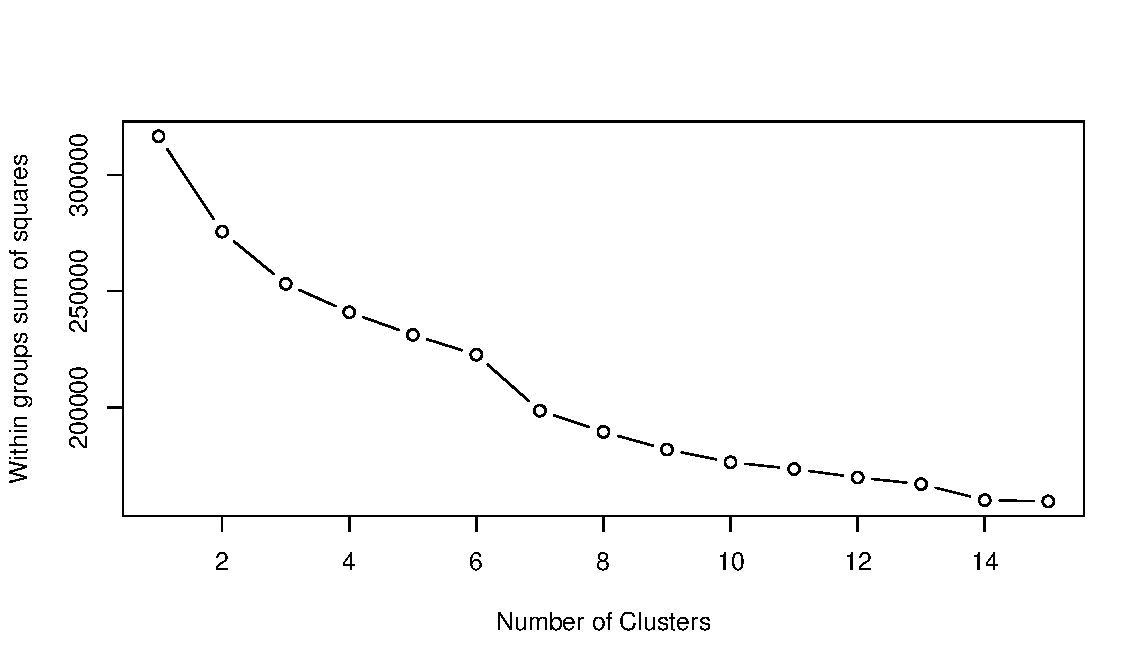
\includegraphics[width=\columnwidth]{figures/cluster_n_1.pdf}
		\end{center}
		\caption{Error de los datos por cada cantidad de clusters \label{fig:cluster_n_1}}%
	\end{figure}

	Ahora con la cantidad de clusters definida podemos aplicar el algoritmo quedando una distribución que tiene una medida de similitud de los elementos dentro de cada cluster de 40.6\%, la cual es baja debido a la cantidad de variables que poseemos sin ninguna correlación entre sí.

	Ahora intentaremos disminuir la dimensión de los datos tomando solo un conjunto de las variables que posee el conjunto de muestras, en particular son las que ya habiamos tomado en los anteriores acercamientos.

	Veamos nuevamente la correlación entre las variables, pero esta vez de las variables seleccionadas.

	\begin{verbatim}
                    m PP PU V n
medIncome           1          
PctPopUnderPov      , 1        
PctUnemployed       , ,  1     
ViolentCrimesPerPop . .  .  1  
nonViolPerPop       . .  .  , 1
	\end{verbatim}

	A pesar de ver un número menor de espacios en blanco, se puede ver como todo son . y , lo que hace que igual no sea un matriz altamente correlacionada, veamos que resultados arroja aplicar el algoritmo de ACP, para esto igualmente estandarizamos los datos. Obtenemos que con solo tomar las dos primeras componentes principales estas obtendriamos una proporción acumulativa de 0.8131 con lo que explicaríamos el 81.31\% de la variación de los datos, este por ciento es mayor que 70\% por lo que es aceptable, esto se puede apreciar mejor en la grafica \ref{fig:acp_2}. Si nos guiásemos por el criterio de Kaiser tenemos que solo la primera componente posee valor propio mayor que 1.

	\begin{figure}[htb]
		\begin{center}
			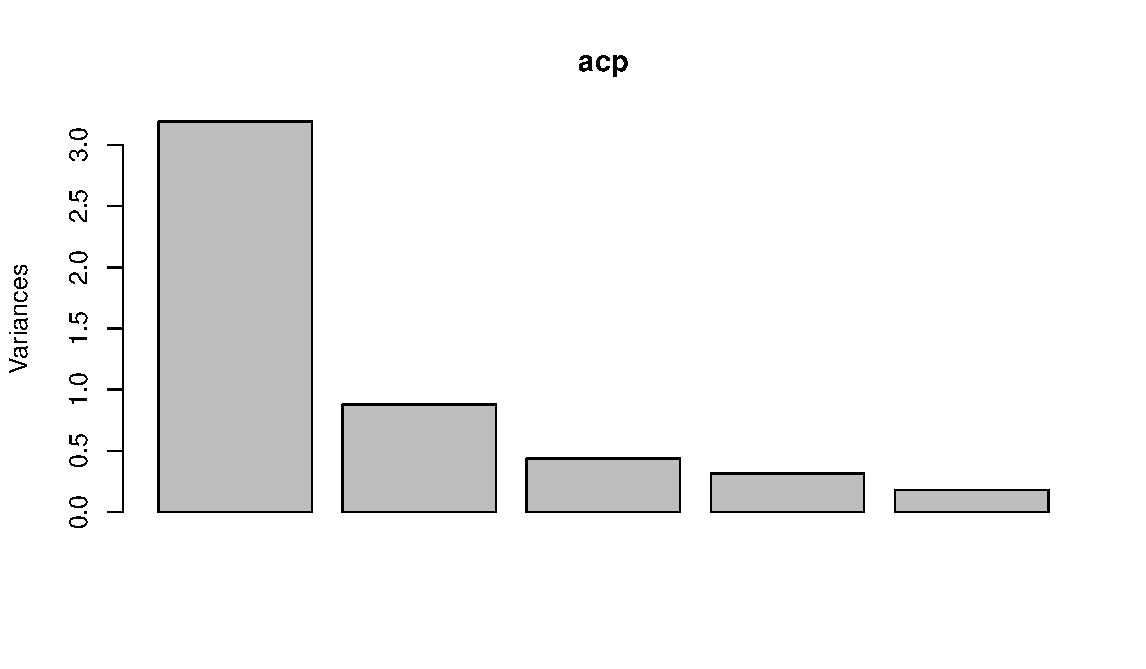
\includegraphics[width=\columnwidth]{figures/acp_2.pdf}
		\end{center}
		\caption{Proporción acumulativa de componentes principales\label{fig:acp_2}}%
	\end{figure}

	Veamos que variables son importantes para la componente 1. Podemos tomar el mayor valor propio absoluto que es 0.5021, teniendo este podemos afirmar que todos los valores propios cuyo módulo esté por encima de 0.2510 en la columna de PC1 son las variables que conforman esta componente. Por tanto PC1 está caracterizada por personas con bajos ingresos, gran porciento de personas por debajo del nivel de pobreza, alto porciento de personas en edad laboral desempleados, alto número de crímenes violentos y alto número de crímenes no violentos.

	Siguiendo el análisis que se realizó teniendo en cuenta todas las variables, podemo aplicar el algoritmo de clústers jerárquicos pero con este obtenemos un resultado similar al anterior en donde se obtiene un clusters que posee a la mayoría de los datos y el resto solo posee una pequeña proporción de las muestras.

	Ahora veamos para este conjunto de variables cuál sería el mejor número de cluster a formar con el algorítmo de K-Means, realizando un análisis similar podemos ver en la gráfica \ref{fig:cluster_n_2} como para estas variables el mejor número de clusters a tomar sería 4. Con esta distribución obtenemos una medida de similitud de los elementos dentro de cada cluster de 69.5\%, la cual es más alta que el anterior análisis a pesar de poseer un menor número de clusters.

	\begin{figure}[htb]
		\begin{center}
			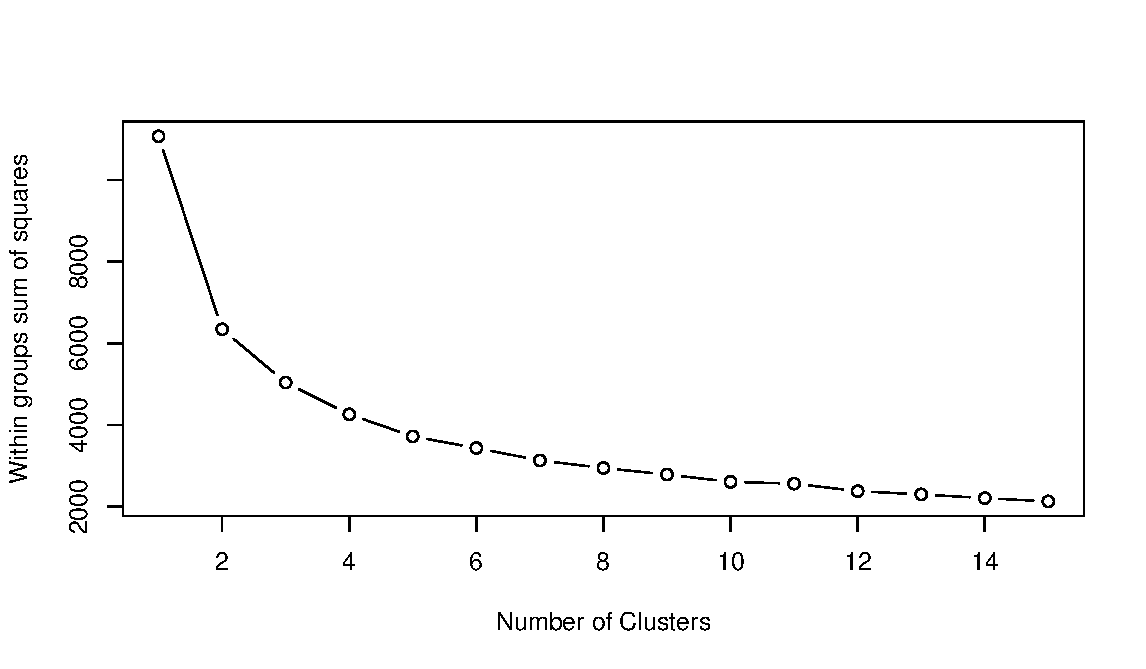
\includegraphics[width=\columnwidth]{figures/cluster_n_2.pdf}
		\end{center}
		\caption{Error de los datos por cada cantidad de clusters \label{fig:cluster_n_2}}%
	\end{figure}

	Podemos ver la distribución de clusters para las muestras con respecto a las variables seleccionadas en la figura \ref{fig:plot_clusters}.

	\begin{figure}[htb]
		\begin{center}
			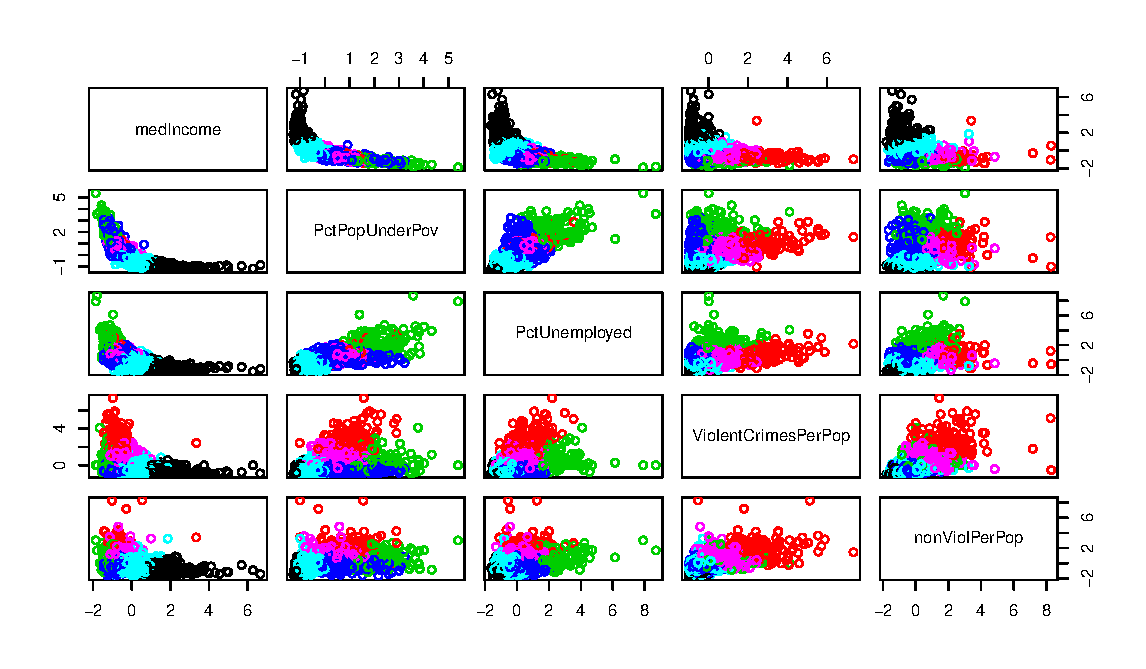
\includegraphics[width=\columnwidth]{figures/plot_clusters.pdf}
		\end{center}
		\caption{Datos representados con colores diferenciando su pertenencia a cada cluster \label{fig:plot_clusters}}%
	\end{figure}
	





%-----------------------------------------------------------------------------------
%-----------------------------------------------------------------------------------
  	
%===================================================================================



%===================================================================================
% Conclusiones
%-----------------------------------------------------------------------------------
\section{Conclusiones}\label{sec:conc}

%===================================================================================



%===================================================================================
% Recomendaciones
%-----------------------------------------------------------------------------------

%===================================================================================



%===================================================================================
% Bibliografía
%-----------------------------------------------------------------------------------
\begin{thebibliography}{99}
%-----------------------------------------------------------------------------------

%-----------------------------------------------------------------------------------
\end{thebibliography}

%-----------------------------------------------------------------------------------

\label{end}

\end{document}

%===================================================================================
